% ----------------------
  \chapter{Diseño del prototipo}



% ----------------------
\section{Etapa de alimentación} \par
Para la alimentación de los amplificadores operacionales que se utilizarán para el sensado de la tensión y corriente, además de los demás componentes que lo requieran, se realiza el diseño de una fuente de continua partida de $\pm 12V$ y una fuente simple de $+5V$ obtenida a partir de los $+12V$ regulados. \par
\begin{figure} [H]
	\centering
	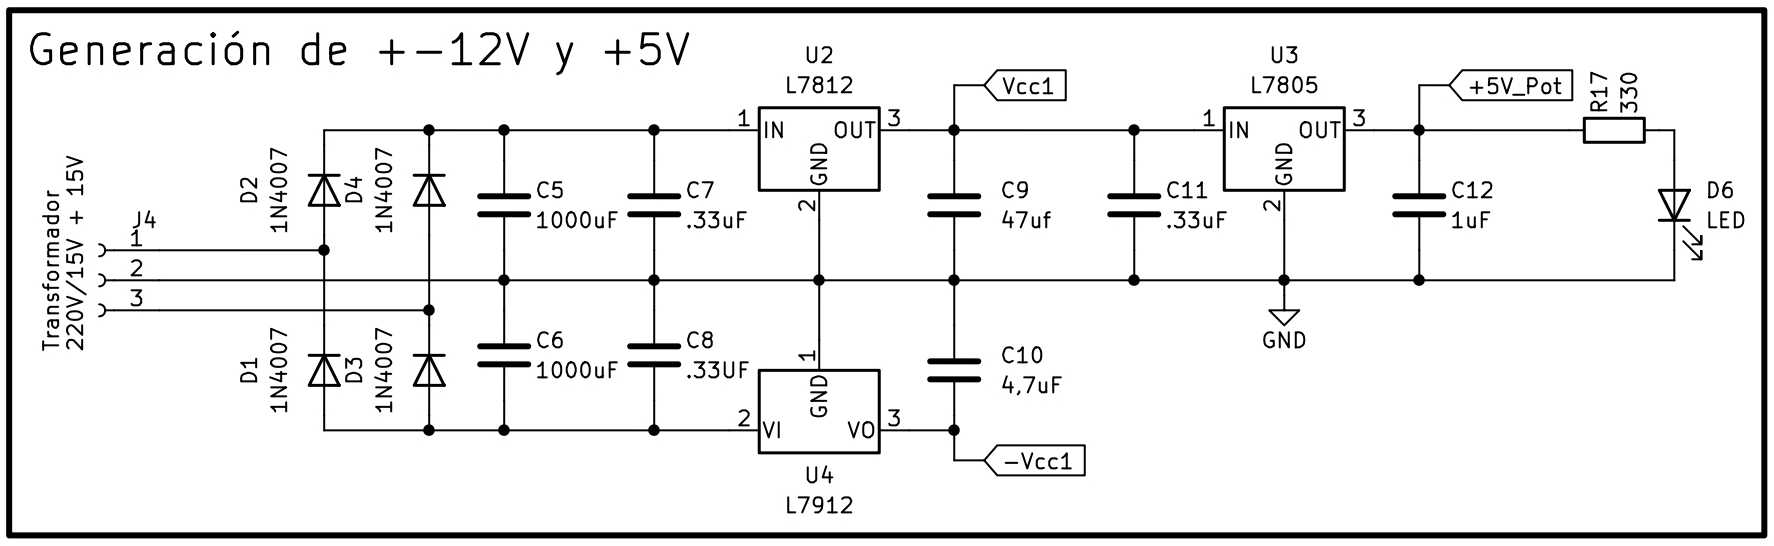
\includegraphics[width=\textwidth]{./imagenes/Alimentacion_analogica.png}
	\caption{Fuente de alimentación de los componentes}
	\label{F:alimentacion_analogica}
\end{figure} \par 
Se cuenta con un transformador de $220V/(15+15)V$. Por lo que definiendo los capacitores $C_5 =C_6 =1000\mu F/25V$ y una corriente máxima supuesta de $500mA$ se tiene una tensión eficaz de \textit{ripple} de:
\begin{equation}
	V_{ripple} =\frac{0,5A}{4\cdot \sqrt{2}\cdot (50Hz)\cdot (1000\mu F)}=1,7677V
\end{equation} \par
Considerando la caída de tensión de un diodo como $V_D =0,7V$ obtenemos la expresión del valor medio de la tensión rectificada:
\begin{equation}
V_{alim} =V_{trafo} \cdot \sqrt{2}-2\cdot V_D -V_{ripple} \cdot \sqrt{2}=(15\cdot \sqrt{2})-(2\cdot 0,7V)-(1,77V\cdot \sqrt{2})=17,31V
\end{equation} \par
En paralelo a los capacitores $C_5$ y $C_6$ se agregan los capacitores $C_7$ y $C_8$ de $0,33\mu F/25V$ para eliminar los ruidos de alta frecuencia según la aplicación recomendada en la hoja de datos del LM78XX [INSERTAR REFERENCIA]. Para los diodos rectificadores se emplean 1N4007.\par
Para fijar el valor de voltaje de salida se emplean los integrados LM7812 y LM7912 de +12V y -12V respectivamente. A continuación se colocan capacitores de desacople con el fin de mejorar la estabilidad y reducir el ruido. Asegurando un suministro de tensión estable y confiable para los demás componentes electrónicos conectados al sistema. \par 
A la salida de la fuente de alimentación de +12V se conecta el regulador, LM7805, para obtener +5V regulados con su correspondiente capacitor de salida de $C_{sal} =1\mu F$. Por ultimo se conecta un LED, en conjunto con una resistencia limitadora, para indicar el correcto funcionamiento de la etapa de alimentación. \par 
\begin{equation}
R_{lim} =\frac{(+5V)-V_{LED} }{I_{LED} }=\frac{(+5V)-(2V)}{10mA}=300\Omega \to 330\Omega
\end{equation} \par 
\begin{equation}
P_{R_{lim} } =\frac{(+5V-2V)^2 }{330\Omega }\cdot 1,5=40,9mW\to 1/8W
\end{equation}

\section{Etapa de Potencia}\par

Para la etapa de potencia se hace uso de un transformador de 220V / 33V siendo el circuito de rectificación y filtrado el que se aprecia a continuación:

\begin{figure} [H]
	\centering
	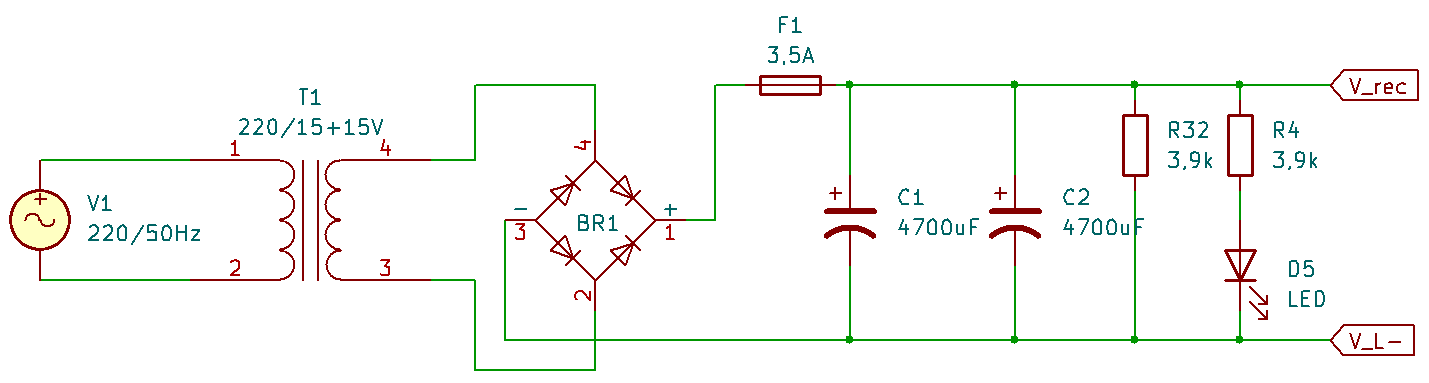
\includegraphics[width=\textwidth]{./imagenes/Rectificador_potencia.png}
	\caption{Circuito de rectificación y filtrado de la etapa de potencia}
	\label{F:rectificador_potencia}
\end{figure} \par 

Se diseña esta etapa para obtener un bajo valor de tensión de \textit{ripple} y que pueda entregar una corriente de 3 A. Para dimensionar el valor del capacitor a utilizar se hace uso de la siguiente expresión:
\begin{equation}
C=\frac{3A}{4\sqrt{2}(50Hz)(\frac{3V/2}{\sqrt{2}})}=1000\mu F
\end{equation} \par 

A partir de este cálculo adoptamos 2 capacitores en paralelo: $C_1 =C_2 =4700~\mu F~/~63~V$, con lo cual la tensión pico a pico de \textit{ripple} resulta de  $V_{r(pp)} =3,1915~V$. \par 

Esto nos da como resultado un valor medio de tensión rectificada y filtrada para una carga de 3 A de: 
\begin{equation}
V_{rec} =(33\cdot \sqrt{2}V)-2\cdot 0,7V-\frac{3,1915V}{2}=43,67V
\end{equation} \par 

Luego, en paralelo a los capacitores se coloca una resistencia $R=3,9k\Omega /1W$ con el fin de descargar los capacitores en un tiempo $\tau =R\cdot C=(3900\Omega )\cdot (2\cdot 4700\mu F)=36,66s$ cuando se desconecte la fuente de alimentación. La corriente a través de la resistencia cuando la carga no sea de $I_0 =3A$ será de:
\begin{equation}
I_{R32} =\frac{V_{rec} }{R32}=\frac{43,67V}{3900\Omega }=11,2mA
\end{equation}\par 

Mientras que la potencia del resistor se calculará empleando un factor de seguridad de $fs=1,5$: 
\begin{equation}
P_R \ge \frac{V_R^2 }{R}\cdot fs=\frac{(43,67V)^2 }{3900\Omega }\cdot 1,5=0,7336W\to 1W
\end{equation} \par 

Adicionalmente se coloca un LED indicativo de encendido con un resistor limitador de valor: 
\begin{equation}
R_{LED} =\frac{V_{rec} -V_{LED} }{I_{LED} }=\frac{43,67V-2V}{10mA}=4167,33\Omega \to 3900\Omega
\end{equation} \par 

\section{Actuador de potencia} \par 

El circuito observado en la Figura \ref{F:Circuito_Actuador} tiene la finalidad de controlar la tensión y corriente de salida. Se denota que se conecta el punto de referencia (GND) a la salida de tensión positiva con el fin de poder utilizar los amplificadores operacionales en torno a este punto de mayor potencial, requiriendo fuentes sencillas de $\pm12V$.

\begin{figure} [H]
	\centering
	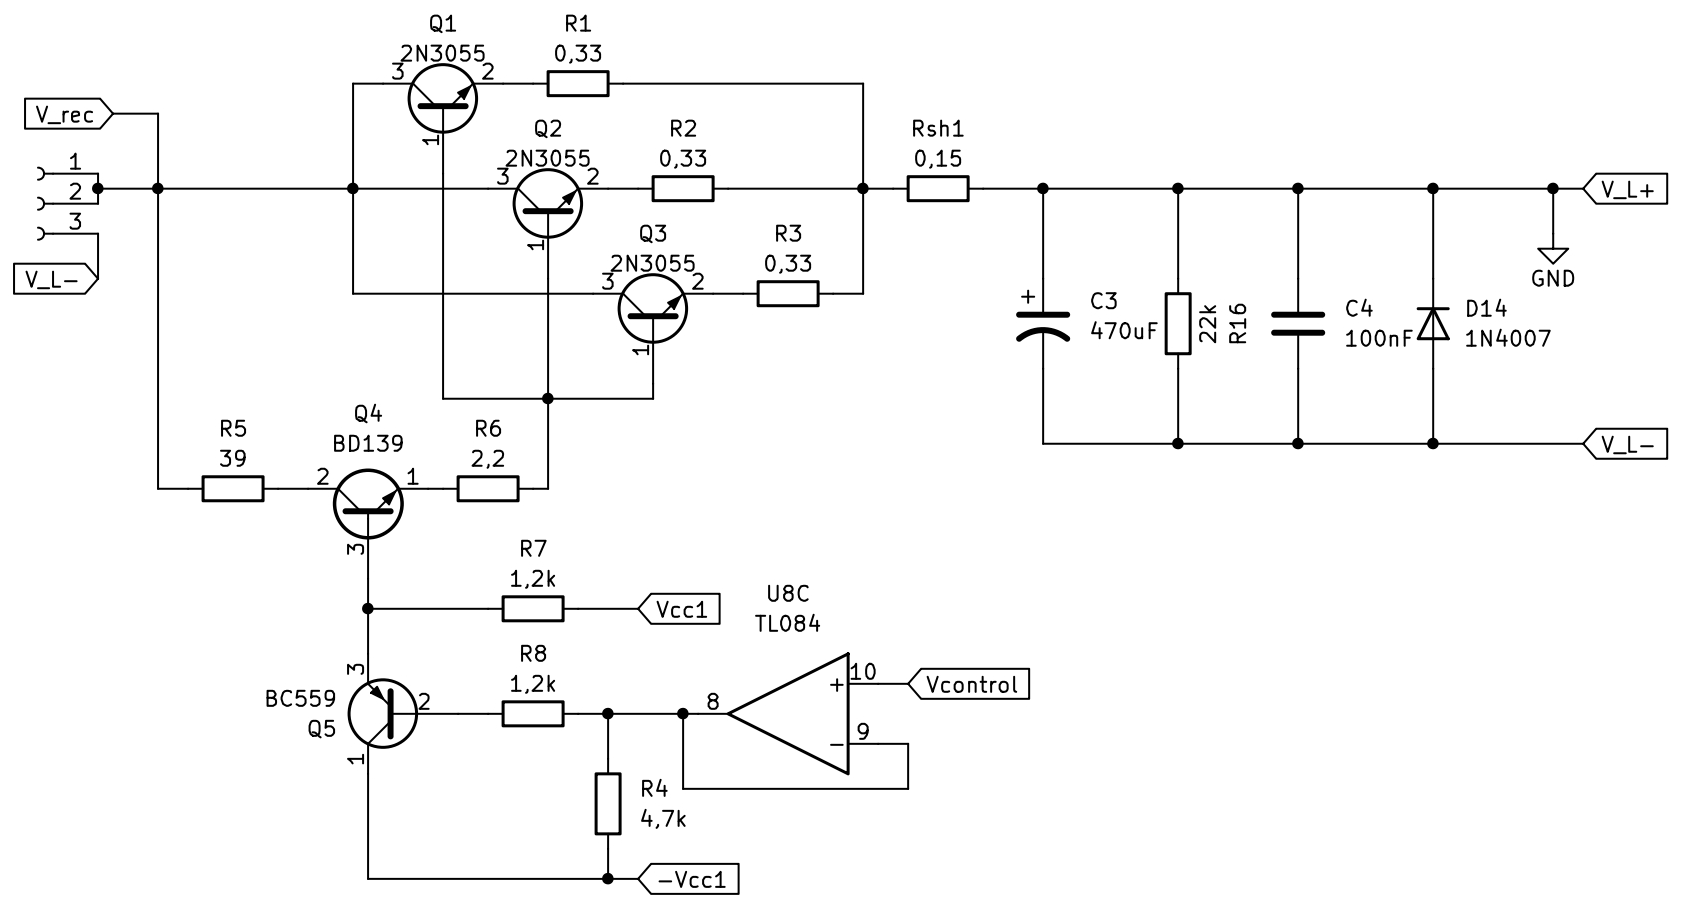
\includegraphics[width=\textwidth]{./imagenes/Circuito_actuador.png}
	\caption{Regulador de tensión con transistores de paso.}
	\label{F:Circuito_Actuador}
\end{figure} \par 

Se utilizó como transistor de potencia tres 2N3055 conectados en paralelo, con ganancia $h_{FE1} =20$ y $V_{BE1(ON)} =1,5~V$ mientras que para accionarlo se utiliza un BD139 con $h_{FE4} =30$ y $V_{BE4(ON)} =1V$. \par 
Considerando el caso de máxima carga $V_L =30V$ y $I_L =3A$ en la base de los transistores debe haber una tensión igual a:
\begin{equation}
\begin{split}
V_{B1}&=V_L+I_L\cdot Rsh1+\frac{I_L}{3}\cdot R1+V_{BE1(on)}= \\
&=(30V)+(3A)\cdot (0,15\Omega)+(1A)\cdot (0,33\Omega)+(1,5V)=32,28V
\end{split}
\end{equation} \par 

Se procede a calcular la corriente de colector a pasar por el transistor BD139 para alcanzar la excitación de los transistores de potencia dada la expresión:
\begin{equation}
I_{C4}=\frac{I_L}{hfe1}=\frac{3A}{20}=0,15A
\end{equation} \par 

Se adopta una resistencia $R6=2,2\Omega$ como resistencia de emisor para estabilización térmica y $V_{CE4}=5V$ para un funcionamiento en zona activa. Por lo que podemos calcular R5 como:
\begin{equation}
R_5=\frac{V_{rec}-V_{CE4}-V_{B1}}{I_C4}-R_6=\frac{43,67 V-5V-32,28V}{0,15A}-2,2\Omega=40,42\Omega \to 39\Omega 
\end{equation} \par 

Verificando las potencias:
\begin{equation}
P_{R5}\geq (0,15A)^2\cdot (39\Omega)\cdot 1,5=1,364 W \to P_{R5}=2W
\end{equation}
\begin{equation}
P_{R6}\geq (0,15A)^2\cdot (2,2\Omega)\cdot 1,5=74,25 mW \to P_{R5}=1/8W
\end{equation} \par

Para el cálculo del disipador del BD139 (Q4) se supone el caso en que ocurre un corto-circuito a la salida de la fuente, actuando el control de corriente manteniendo estable la corriente en $I_L=3A$ y la tensión $V_L=0V$. Por lo que la tensión de colector-emisor de Q4 será:
\begin{equation}
\begin{split}
V_{CE4max}&=V_{rec}-I_{C4}\cdot (R5+R6)-V_{B1}=\\
&=43,67V-0,15A\cdot (39+2,2)\Omega -2,28V=35,21 V
\end{split}
\end{equation} \par 

Se calcula la potencia que debe disipar el transistor Q4:
\begin{equation}
\begin{split}
P_{Q4}&=V_{CE4(max)}\cdot I_{C(max)}+V_{BE(on)}\cdot \frac{I_{C(max)}}{hfe4}=\\
&=35,21V\cdot 0,15A+1V\cdot \frac{0,15A}{40}=5,28W
\end{split}
\end{equation} \par 

Como la potencia que debe disipar es mayor a la que puede soportar sin disipador ($1 W$ extraído de la hoja de datos), resulta necesario dimensionar un disipador. Para ello se emplea la temperatura de juntura máxima ($T_{J4}=150^\circ C$), la resistencia térmica juntura-carcasa para el encapsulado TO-126 ($\theta _{JC}=10^\circ C/W$), la resistencia térmica carcasa-disipador (en este caso, pasta térmica $\theta _{CD}=1^\circ C/W$) y se supone una temperatura ambiente $T_A=50^\circ C$. Por lo que la resistencia térmica disipador-ambiente debe ser igual o menor que:
\begin{equation}
\begin{split}
\theta_{DA} &= \frac{T_J-T_A}{P_{Q4}}-\theta_{JC}-\theta_{CD}=\\
&= \frac{(150-50)^\circ C}{5.28W}-(10^\circ C/W)-(1^\circ C/W)=7.92^\circ C/W
\end{split}
\end{equation} \par
 
A continuación se procede a calcular las resistencias R7, R8 y R9. Para R7 se supone el caso de $V_L=30 V$ y $I_L=3 A$ donde la corriente de colector del transistor Q4 es de $I_{C4}=150 mA$. Dada una ganancia de $hfe4=40$ la corriente de base de este transistor será:
\begin{equation}
I_{B4}=\frac{I_{C4}}{hfe4}=\frac{150mA}{40}=3,75mA
\end{equation}\par

Suponiendo que la corriente de emisor de Q5 es igual a la corriente de base de Q4, es decir $I_{E5}=I_{B4}=3,75mA$, tenemos que la corriente a través de R7 será $I_{R7}=I_{B4}+I_{E5}=7,5mA$. Paso siguiente, se determina la tensión en la base de Q4:
\begin{equation}
V_{B4}=V_{B1}+I_{C4}\cdot R_6+V_{BE4}=32,28V+(0,15A\cdot 2,2\Omega)+1V=33,61V
\end{equation}\par

Debido a que el punto de referencia ($GND=0V$) de la fuente de $\pm 12V$ coincide con el borne positivo de $V_{L+}$ de la fuente de salida de $V_L=30V$, entonces el nivel de tensión de $V_{cc1}$ respecto al borne negativo $V_{L-}$ es de $V'_{cc1}=V_{cc1}+V_L=12V+30V=42V$. Por lo que la resistencia R7 puede calcularse como:
\begin{equation}
R7=\frac{V_{cc1}-V_{B4}}{I_{R7}}=\frac{42V-33,61V}{7,5 mA}=1118 \Omega \to 1200\Omega
\end{equation}\par 

Para el cálculo de R8 establecemos que $I_L=0A$ de modo que la base de Q4 tenga un potencial próximo a los $0V$, donde podemos adoptar un potencial de aproximadamente $0,8V$. Esto provoca que el BD139 esté en corte, y la tensión y corriente de salida sean nulas. Por lo que en este caso, toda la corriente que circula a través de R7 corresponde a la corriente de emisor de Q5. Por lo que:
\begin{equation}
I_{R7(max)}=\frac{V_{cc1}-V_{B4(min)}}{R7}=\frac{12V-0,8V}{1200}\cong 9,33 mA
\end{equation} \par 
El transistor Q5 es un BC559 y tiene una ganancia $hfe5=110$ y una tensión emisor-base $V_{EB5}=0,7V$ con la cual la resistencia R8 resulta:
\begin{equation}
R8=\frac{V_{B4}-V_{EB5}}{(\frac{I_{R7}}{hfe5})}=\frac{0,8V-0,7V}{(\frac{9,33 mA}{110})}=1178,57\Omega \to 1200\Omega
\end{equation}\par 

La resistencia R9 es una resistencia de \textit{pull-down} que tiene la utilidad de dejar establecido un valor de tensión a la base de Q5 en caso que se desconecte el controlador. Por lo tanto, podemos calcular su valor suponiendo que por la misma no va a circular más que unos $I_{R9}=2,5 mA$ cuando el voltaje en el punto superior se encuentre a $0V$.
\begin{equation}
R9=\frac{V_C-(-V_{cc1})}{I_R9}=\frac{0V-(-12V)}{2,5 mA}=4800\Omega \to 4700\Omega 
\end{equation}\par 

A continuación se calcula las potencias a disipar por las resistencias R7, R8, R9 y el transistor Q5. Se consideran los escenarios donde circula la mayor corriente, donde para R9 se puede suponer un caso extremo de $V_{B(extremo)}=-12V$. Mientras que para el transistor se supone $V_{CE5(max)}=5V$:
\begin{equation}
P_{R7}\geq (9,33mA)^2\cdot (1200\Omega )\cdot 1,5=156,8 mW	\to P_{R7}=1/4W
\end{equation}
\begin{equation}
P_{R8}\geq (\frac{9,33mA}{110})^2\cdot (1200\Omega )\cdot 1,5= 13\mu W \to P_{R8}=1/8W
\end{equation}
\begin{equation}
P_{R9}\geq \frac{(12V-0V)^2}{1200\Omega}\cdot 1,5=183,82 mW	\to 	P_{R9}=1/4W
\end{equation}
\begin{equation}
P_{Q5}=(5V\cdot 9,33mA)+0,7V\cdot \frac{9,33mA}{110}\cong 46,73mW
\end{equation}\par 

De la hoja de datos de Q5 tenemos que $P_{Q5(max)}=500mW$, por lo que se cumple que $P_{Q5}<P_{Q5(max)}$. Respecto a la potencia disipada en R1, R2 y R3 que se corresponden con las resistencias de emisor de los transistores de potencia, su corriente máxima será de $I_{L(max)}/3=1A$, por lo que:
\begin{equation}
P_{R1}\geq (1A)^2\cdot (0,33\Omega)\cdot 1,5=495 mW \to P_{R1}=P_{R2}=P_{R3}=1W
\end{equation}\par 
La máxima disipación de potencia en los transistores Q1, Q2 y Q3 está dado para el caso de $I_L=3A$ cuando $V_L=0V$, que ocurre ante un cortocircuito a la salida. En este caso, tenemos una tensión (despreciando caída en diodos rectificadores) de $V_{CE1} = (43,67 V)-(0,33 V)-(0,45 V)=42,89 V$ y una corriente de colector de $I_{C1(max)}=1 A-(1A/20)=950mA$. Por lo que la potencia que disipa será:
\begin{equation}
P_{Q1}=(42,89V\cdot 0,95A)+1,5V\cdot \frac{0,95A}{20}=40,82 W
\end{equation}\par 
Se calcula si el transistor podrá disipar esa potencia sin disipador conociendo que su resistencia térmica de juntura-ambiente es de $\theta _{JA}=20^\circ C/W$ y la temperatura máxima de juntura es $T_J=200^\circ C$ y la temperatura ambiente se establece en $T_A=50^\circ C$.
\begin{equation}
P_{Q1(SD)}=\frac{(200-50)^\circ C}{20^\circ C/W}=7,5W \to P_{Q1}>P_{Q1(SD)} \to \text{Requiere disipador}
\end{equation} \par 
Se dimensiona el disipador conociendo que la resistencia térmica juntura-carcasa es $\theta_{JC}=1,5^\circ C/W$ y la resistencia térmica carcasa-disipador es $\theta_{CD}=0,5^\circ C/W$ (contacto con grasa y arandela de mica).
\begin{equation}
\theta_{DA1}=\frac{(200-50)^\circ C}{40,82 W}-(10^\circ C/W)-(0,5^\circ C/W)=1,655^\circ C/W
\end{equation}
Por lo que se requiere un disipador con una resistencia térmica igual o menor que $\theta_{DA1}=1,655^\circ C/W$.


\section{Sensado de corriente}
En esta etapa se emplea una resistencia de \textit{Shunt} $R_{sh1} =0,15~\Omega$ para obtener un voltaje proporcional a la corriente que está circulando por la misma. Luego para elevar el valor del mismo en torno a los 5 V cuando estén circulando 3 A por la misma se utiliza un amplificador operacional en una configuración de amplificador no inversor, dada por la siguiente expresión:
\begin{equation}
V_{o1} =V_{NI} \times (1+\frac{R_{V4} }{R_{14} })=(I_L \times R_{sh1} )\times (1+\frac{R_{V4} }{R_{14} })
\end{equation}\par 

\begin{figure} [H]
	\centering
	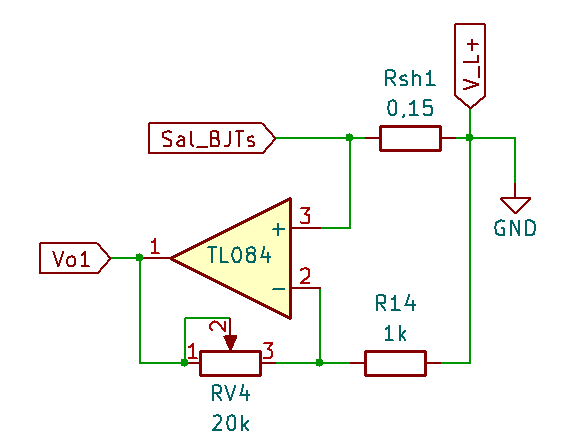
\includegraphics[width=0.6\textwidth]{./imagenes/Sensor_corriente.png}
	\caption{Circuito de sensado de la corriente de salida}
	\label{F:Sensor_corriente}
\end{figure} \par 

Cuando circule $I_L =3A$ por $R_{sh1}$ obtendríamos un voltaje en la entrada no inversora de $V_{NI} =3A\cdot 0,15\Omega =0,45V$ por lo que adoptando el resistor $R_{14} =1k\Omega$ y calibrando el potenciómetro $R_{V4} $ a $10k\Omega$ obtenemos como resultado para fondo de escala una tensión de:
\begin{equation}
V_{o1} =(0,45V)\cdot (1+\frac{10k\Omega }{1k\Omega })=4,95V
\end{equation} \par 

Se coloca el preset RV4 con el fin de poder calibrar el voltaje de salida $V_{o1}=5V$ para una corriente $I_L=3A$. Las potencias de las resistencias se obtienen como:
\begin{equation}
P_{Rsh1}\geq I_L^2\cdot Rsh1\cdot 1,5=(3 A)^2\cdot (0,15 \Omega)\cdot 1,5\cong 2 W \to P_{Rsh1}=2W
\end{equation}
\begin{equation}
P_{R14}\geq \frac{V_I^2}{R_{14}}\cdot 1,5=\frac{(0,45 V)^2}{1000\Omega}\cdot 1,5 \cong 0,3 mW \to P_{R14}=1/8W
\end{equation} \par

\section{Sensado de tensión}
Se requiere un circuito que convierta los niveles de tensión de la salida. Para ello se presenta el circuito a continuación, en el cual se puede variar la ganancia del sistema ajustando el potenciómetro RV1.
\begin{figure} [H]
	\centering
	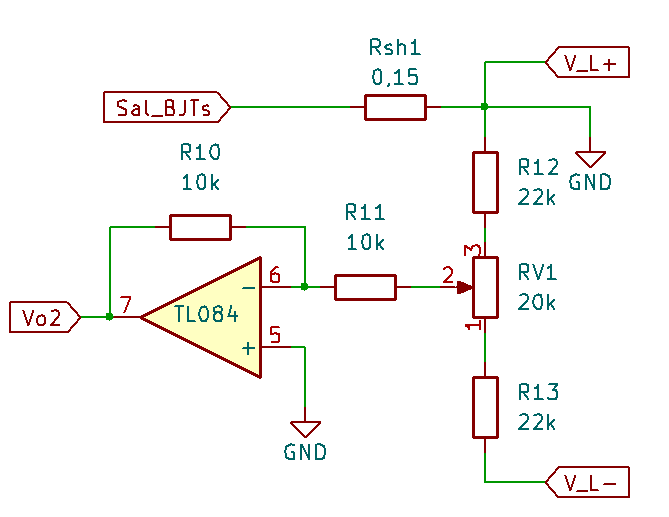
\includegraphics[width=0.6\textwidth]{./imagenes/Sensor_tension.png}
	\caption{Circuito de sensado de la tensión de salida}
	\label{F:Sensor_tension}
\end{figure} \par 

Debido a que el punto común de referencia ($0 V$) de las fuentes de $\pm 12V$ coincide con el borne positivo $V_{L+}$ de salida de la fuente lineal, el borne opuesto respecto a GND será de hasta $V_{L-}=-30V$. Como el valor leído desde el cursor de RV1 es negativo, para poder ser comparado con la referencia es necesario invertir su signo mediante un amplificador inversor con ganancia unitaria. \par 

Estableciendo el valor de las resistencias $R_{12}=R_{13}=22k\Omega$ y despreciando la corriente que fluye a través del cursor del preset RV1 hacia la entrada de alta impedancia del amplificador operacional, la corriente a través de $R_{12}$, $R_{13}$ y $RV1$ para $V_L=30V$ será de:
\begin{equation}
I_{R12}=\frac{V_L}{R12+RV1+R13}=\frac{30 V}{(2\cdot 22000+20000)\Omega}\cong 469\mu A
\end{equation} \par 

Por lo tanto, las potencias resultan de
\begin{equation}
P_{R12}\geq (I_{R12})^2\cdot R12\cdot fs=(469\mu F)^2\cdot (22000 \Omega)\cdot 1,5 \cong 7,6 mW \to P_{R12}=P_{R13}=P_{RV3}=1/8W
\end{equation} \par 

Mientras que se definen las resistencias $R10=R11=10 k\Omega \ 1/8W$ debido a que la corriente que circulan por ellas es despreciable.\par 



\section{Acople y desacople de carga}
Para conectar y desconectar la carga se utiliza un relé de salida. El mismo será accionado cuando el usuario lo determine luego de establecer los valores deseados de tensión y/o corriente de salida. El circuito puede apreciarse en la Figura \ref{F:Circuito_Acople_carga}.

\begin{figure} [H]
	\centering
	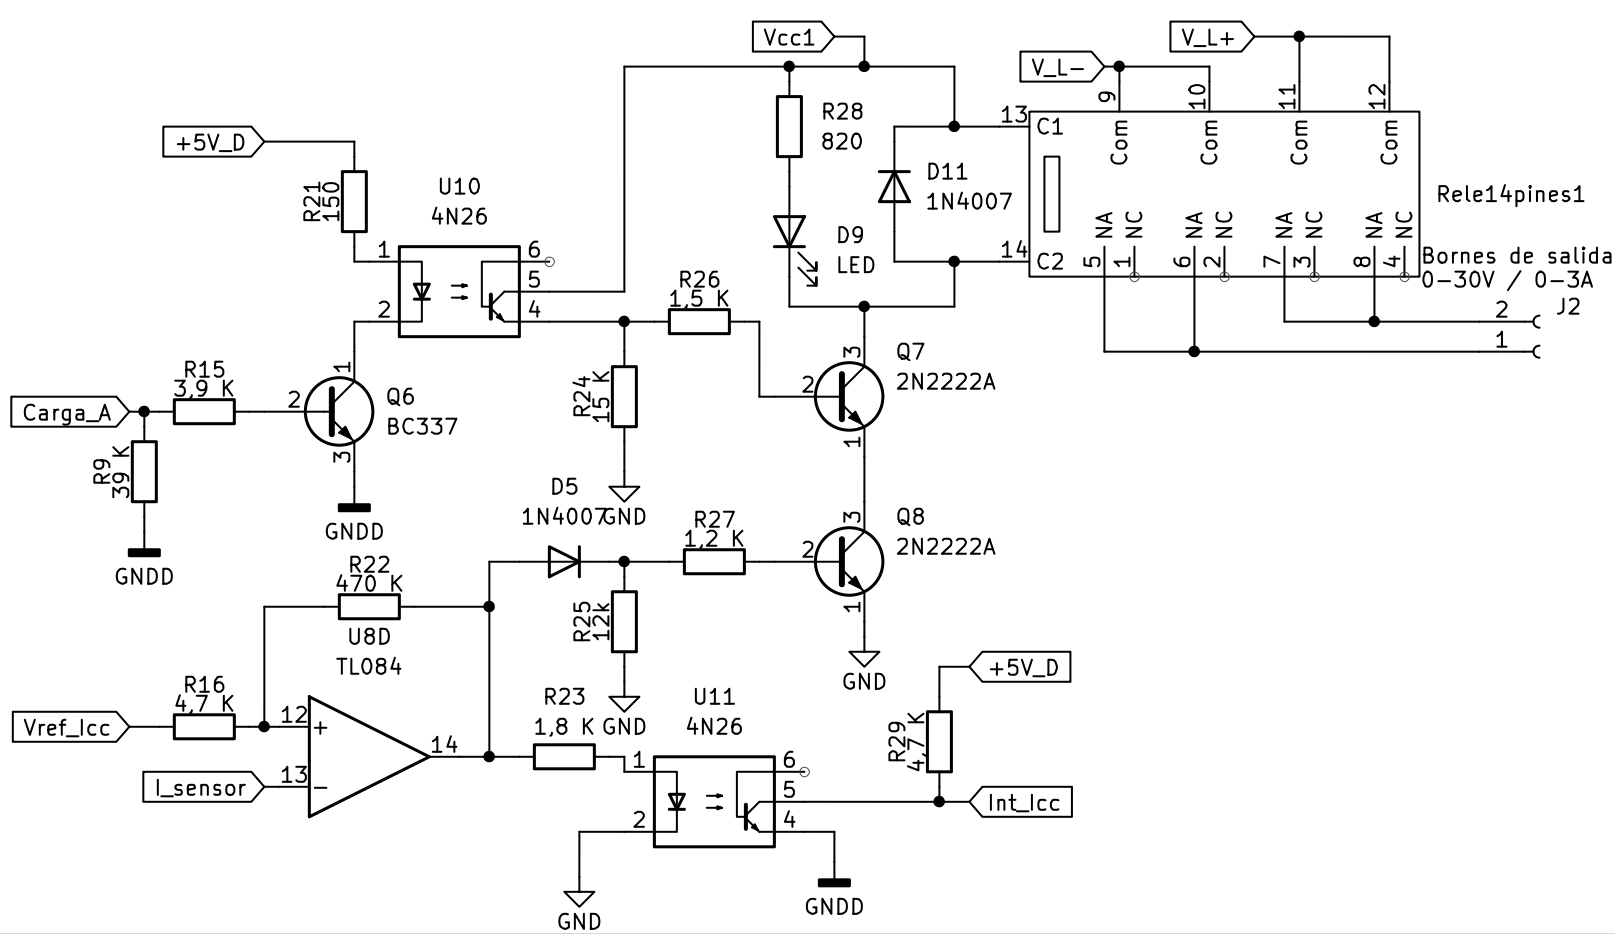
\includegraphics[width=\textwidth]{./imagenes/Acople_carga.png}
	\caption{Circuito de acople y desacople de carga.}
	\label{F:Circuito_Acople_carga}
\end{figure} \par 

Como transistor se utiliza el 2N2222A \cite{2N2222}, el cual soporta las siguientes magnitudes: $V_{CEmax}=40V$; $I_{Cmax}=600 mA$ y $P_{Dmax}=625 mW$. Las características de funcionamiento que presenta son $V_{CE(sat)}=0,3V$; $V_{BE(on)}=1,2V$ y $hfe=100$

\begin{equation}
R_{LED}=\frac{V_{cc1}-V_{LED}-2\cdot V_{CE(sat)}}{I_LED}=\frac{12V-2V-2\cdot 0,3V}{10 mA}=940\Omega \to 820 \Omega
\end{equation}
\begin{equation}
I_{LED}=\frac{V_{cc1}-V_{LED}-2\cdot V_{CE(sat)}}{R_LED}=\frac{12V-2V-2\cdot 0,3V}{820 \Omega}=11,46 mA
\end{equation}
Considerando que la corriente que circula por la bobina del Relé es de $30 mA$, se calculan las resistencias de base de la siguiente manera:
\begin{equation}
I_C=I_{Rele}+I_{LED}=30mA+11,46 mA=41,46 mA
\end{equation}
\begin{equation}
I_B=5\cdot \frac{I_C}{hfe}=5\cdot \frac{41,46 mA}{100}=2,073 mA
\end{equation}
\begin{equation}
	R_{BQ7}=\frac{V_{cc1}-V_{CE(Opto)}-V_{CE(Q8)}-V_{BE(Q7)}}{I_B}=\frac{12V-0,5V-0,3V-1,2V}{2,073mA}=4823 \Omega
\end{equation}
\begin{equation}
	R_{BQ8}=\frac{V_{OH}-V_D-V_{BE(Q7)}}{I_B}=\frac{10V-0,7V-1,2V}{2,073 mA}=3907 \Omega
\end{equation}

Se adopta $R_{BQ7}=1,5 k\Omega$ y $R_{BQ8}=1,2 k\Omega$ para asegurar la saturación. Además se agregan las resistencias R24 y R25 con el fin de que la base de los transistores se mantenga con un nivel de tensión bajo cuando se desea que los mismos permanezcan en corte.\par 
El amplificador operacional TL084 \cite{TL084} que se observa en la Figura \ref{F:Circuito_Acople_carga} se encuentra en la configuración de comparador con histéresis. El mismo se encarga de comparar el voltaje correspondiente a la corriente de salida con un valor de referencia $V_{ref(icc)}$ establecido por el usuario. Este cumple la función de que ante un caso extremo de corriente, desacoplar la carga por seguridad. Además, acciona una interrupción en el microcontrolador indicando el error.\par 


















